\documentclass[14pt, aspectratio=169, handout]{beamer}
\usetheme{Copenhagen}
\usecolortheme{seahorse}
\setbeamertemplate{navigation symbols}{}
\setbeamertemplate{headline}{}

%\usepackage{pgfpages}
%\pgfpagesuselayout{4 on 1}[a4paper, border shrink=5mm]

\usepackage{graphicx} % Required for inserting images
\usepackage{multicol}
%\usepackage{enumitem}
\usepackage{amsfonts}
\usepackage{amsmath}
\usepackage{xcolor}

\definecolor{darkblue}{RGB}{0, 0, 139}
\definecolor{lightblue}{RGB}{173, 216, 230}

\title{SST1 Übungsstunde 3}
\author{Matteo Dietz}
\date{September 2025}

\begin{document}

\maketitle

\begin{frame}{Organisatorisches}
    \begin{itemize}
        \item Vorlesungsskript und Übungsskript auf der Vorlesungswebsite
        \item[] Username: sigsys2025, \hspace{10pt} Passwort: Fourier2025
        \item[] 
        \item Link zu meinen Handouts ebenfalls auf der Vorlesungswebsite
    \end{itemize}
\end{frame}

\begin{frame}{Themenüberblick}
    \begin{itemize}
        \item \textbf{Systeme und Systemeigenschaften:}
        \item[] Linearität, Nullraum und Bildraum, Stetigkeit
        \item[] Das inverse System
        \item[] Darstellung linearer Systeme über Matrizen
        \item[] 
        \item \textbf{Eigenschaften zeitkontinuierlicher linearer Systeme}
        \item[] Zeitinvarianz, Kausalität, Gedächtnis, BIBO-Stabilität
    \end{itemize}
\end{frame}

\begin{frame}{Aufgaben für diese Woche}
    \begin{itemize}
        \item[] 25, 26, \underline{\textbf{27}}, \underline{\textbf{28}}, \underline{\textbf{29}}, 30, \underline{\textbf{32}}
        \item[] 
        \item[] Die \underline{\textbf{fettgedruckten}} Übungen empfehle ich, weil sie wesentlich zu eurem Verständnis der Theorie beitragen und/oder sehr prüfungsrelevant sind.
    \end{itemize}
\end{frame}

\begin{frame}{Repetition: Systeme}
    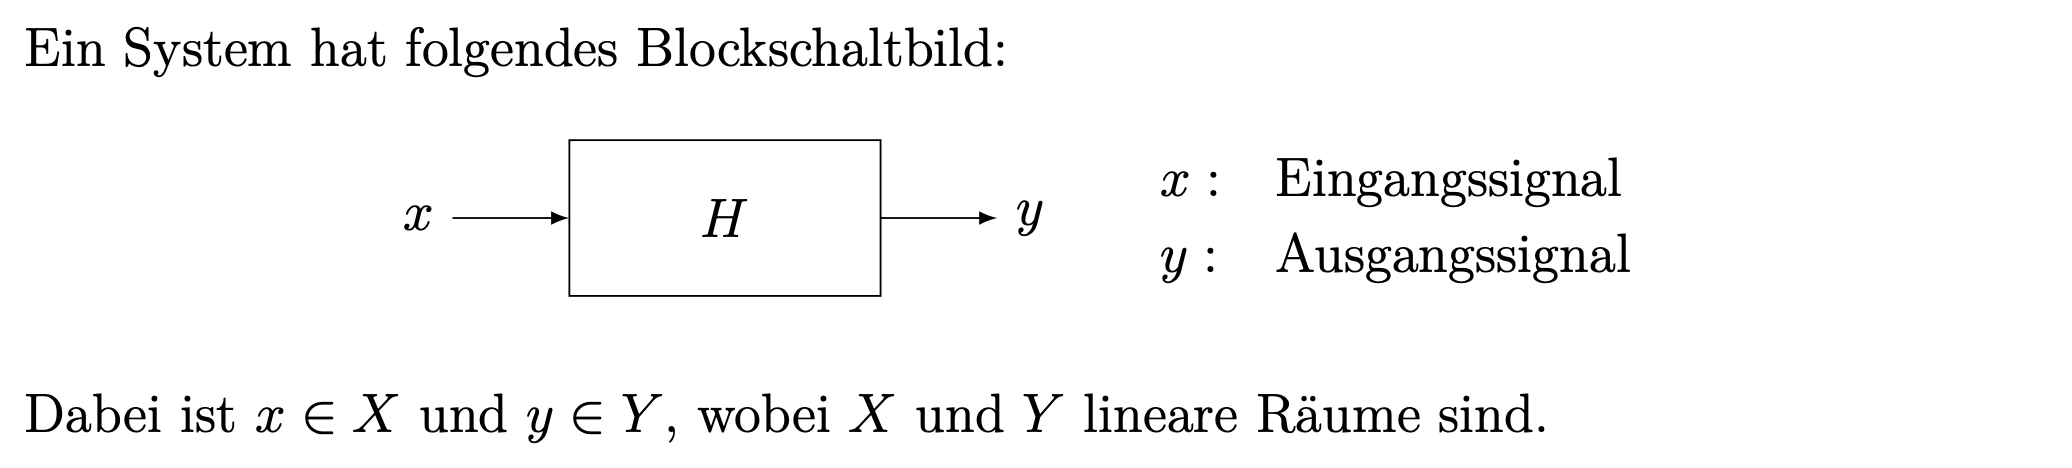
\includegraphics[width=1.1\linewidth]{figures/System_Blockschaltbild.png}
\end{frame}

\begin{frame}{Repetition: Linearität}
    \begin{itemize}
        \item Ein System $H:X \to Y$ ist \textbf{linear}, wenn:
        \item[] \begin{itemize}
            \item[] 
            \item[(i)] \textbf{Additivität}: $H(x_1 + x_2) = Hx_1 + Hx_2$, für alle $x_1,x_2 \in X$
            \item[] 
            \item[(ii)] \textbf{Homogenität}: $H(\alpha x) = \alpha H x$, für alle $x\in X$ und alle $\alpha \in \mathbb{C}$
        \end{itemize}
        \item[]  
        \item Falls das System $(i) \lor (ii)$ nicht erfüllt, heisst $H$ \textbf{nichtlinear}.
    \end{itemize}  
\end{frame}

\begin{frame}{Repetition: Linearität}
    \begin{itemize}
        \item Wenn $H$ ein lineares System ist, dann muss $H0 = 0$ immer gelten.
        \item[] 
        \item Wenn dies also nicht erfüllt ist, dann muss $H$ nichtlinear sein.
    \end{itemize}
\end{frame}

\begin{frame}{Nullraum}
    \begin{itemize}
        \item Sei $H:X \to Y$ ein lineares System
        \item[] 
        \item[] Der Nullraum von $H$ ist die Teilmenge von $X$ definiert durch $\mathcal{N}(H) = \{x \in X : Hx = 0\}$.
        \item[] 
        \item[] $\mathcal{N}(H)$ ist ein linearer Unterraum von $X$.
        \item[] 
        \item[] 
        \item[] 
    \end{itemize}
\end{frame}

\begin{frame}{Bildraum}
    \begin{itemize}
        \item Sei $H:X \to Y$ ein lineares System
        \item[] 
        \item[] Der Bildraum von $H$ ist die Teilmenge von $Y$ definiert durch $\mathcal{R}(H) = \{y =Hx : x \in X\}$.
        \item[] 
        \item[] $\mathcal{R}(H)$ ist ein linearer Unterraum von $Y$.
        \item[] 
        \item[] 
        \item[] 
    \end{itemize}
\end{frame}

\begin{frame}{Nullraum und Bildraum}
    \begin{center}
        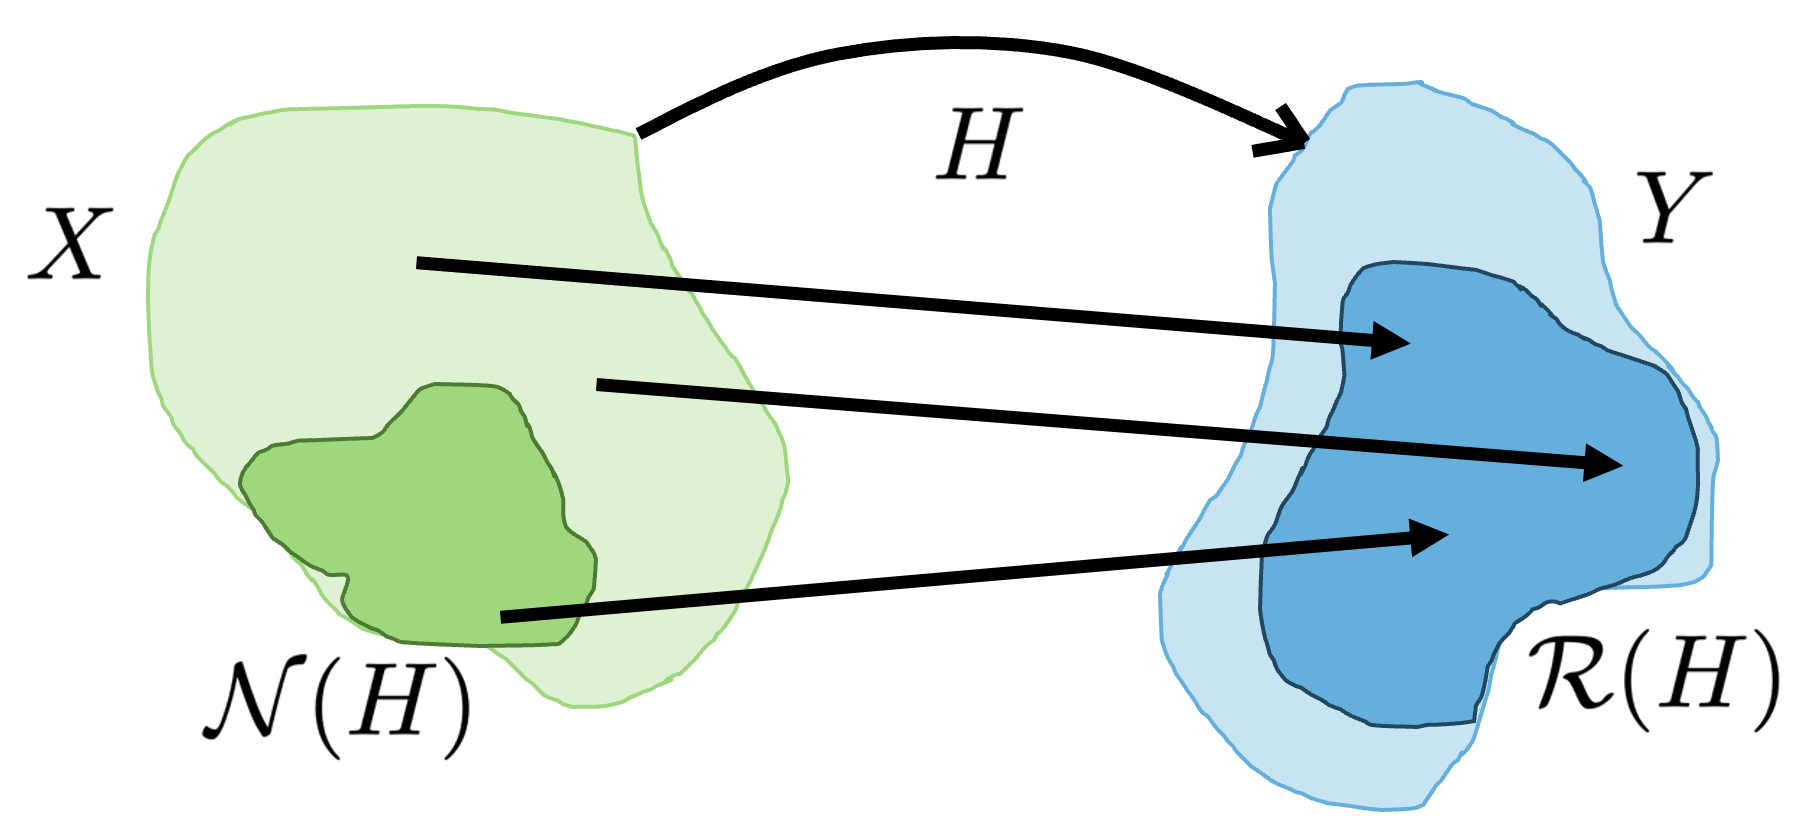
\includegraphics[width=0.9\linewidth]{figures/Bildraum_Nullraum.png}
    \end{center}
\end{frame}

\begin{frame}{Stetige Systeme}
    \begin{itemize}
        \item \textbf{Theorem:} Das System $H$ ist \textbf{linear und stetig}
        \item[] \hspace{64pt}  $\Leftrightarrow$ Für jede konvergente Reihe $\sum_{i=1}^\infty \alpha_i x_i$ gilt:
        \item[] 
    $$H\left( \sum_{i=1}^\infty \alpha_i x_i \right) = \sum_{i=1}^\infty \alpha_i H x_i$$
    \end{itemize}
\end{frame}

\begin{frame}{$\varepsilon-\delta$ Stetigkeit}
    \begin{itemize}
        \item Seien $(X, ||\cdot||))$ und $(Y, ||\cdot||))$ normierte lineare Räume.
        \item[] 
        \item[] Das System $H:X \to Y$ ist \textbf{stetig} in $x_0 \in X$, falls es zu jedem $\varepsilon > 0$ ein nur von $\varepsilon$ abhängiges $\delta >0$ gibt, so dass:
        \item[] 
        \item[] $\forall x\in X$ mit $||x-x_0||<\delta$ folgt, dass $||Hx-Hx_0||\leq \varepsilon$.
    \end{itemize}
\end{frame}

\begin{frame}{Das Inverse System}
    \begin{itemize}
        \item $H:X \to Y$ ist \textbf{invertierbar}, wenn $G:Y \to X$ existiert, sodass: $GH = I_X$ und $HG = I_Y$, 
        \item[] 
        \item[] wobei $I_X$ bzw. $I_Y$ die Identitätsabbildungen auf $X$ bzw. $Y$ sind. (D.h. $I_X x = x$, für alle $x\in X$ und $I_Y y= y$, für alle $y \in Y$.) 
        \item[] 
        \item Man schreibt $H^{-1} = G$.
    \end{itemize}
\end{frame}

\begin{frame}{Das Inverse System}
    \begin{itemize}
        \item Wenn ein System invertierbar ist, dann ist seine Inverse \textbf{eindeutig}.
        \item[] 
        \item[]
        \item[] 
        \item[]
        \item[] 
        \item[]
    \end{itemize}
\end{frame}

\begin{frame}{Das Inverse System}
    \begin{itemize}
        \item Die Inverse eines linearen Systems ist auch linear.
        \item[] 
        \item[]
        \item[] 
        \item[]
        \item[] 
        \item[]
    \end{itemize}
\end{frame}

\begin{frame}{Darstellung linearer Systeme über Matrizen}
    \begin{itemize}
        \item Wir betrachten allgemeine endlich-dimensionale lineare Systeme $H:X \to Y$ und beschreiben diese durch eine Matrix.
        \item[] 
        \item Die linearen Räume $X$ und $Y$ haben als Basen $B_1 = \{x_1, \dots, x_n\}$ und $B_2 = \{ y_1, \dots, y_m \}$.
        $$x = \alpha_1 x_1 + \dots + \alpha_n x_n$$
        $$y = \beta_1 y_1 + \dots + \beta_m y_m$$
    \end{itemize}
\end{frame}

\begin{frame}{Darstellung linearer Systeme über Matrizen}
    
\end{frame}

\begin{frame}{Darstellung linearer Systeme über Matrizen}
    
\end{frame}

\begin{frame}{Darstellung linearer Systeme über Matrizen}
    \begin{itemize}
        \item In Matrixform:
        \item[] 
    \end{itemize}
    $$\begin{bmatrix}
        \beta_1 \\ \beta_2 \\ \vdots \\ \beta_m
    \end{bmatrix} = \underbrace{\begin{bmatrix}
        t_{11} & t_{12} & \dots & t_{1n} \\
        t_{21} & t_{22} & \dots & t_{2n} \\
        \vdots & \vdots & \ddots & \vdots \\
        t_{m1} & t_{m2} & \dots & t_{mn} \\
    \end{bmatrix}}_{\mathbf{H}} \cdot \begin{bmatrix}
        \alpha_1 \\ \alpha_2 \\ \dots \\ \alpha_n
    \end{bmatrix}$$
    \begin{itemize}
        \item Die $m \times n$ Matrix $\mathbf{H}$ stellt das System $H$ in den Basen $B_1$ und $B_2$ dar.
    \end{itemize}
\end{frame}

\begin{frame}{Aufgabe 25 \& 26}
    
\end{frame}

\begin{frame}{Eigenschaften zeitkontinuierlicher linearer Systeme}
    \begin{itemize}
        \item Zeitinvarianz
        \item[] 
        \item Kausalität
        \item[] 
        \item Gedächtnis
        \item[] 
        \item BIBO-Stabilität
    \end{itemize}
\end{frame}

\begin{frame}{Zeitinvarianz}
    \begin{itemize}
        \item \textbf{Definition}: Ein System $H:X \to Y$ ist \textbf{zeitinvariant}, wenn
        $$HT_\tau x = T_\tau Hx, \text{ für alle } x \in X, \; \tau \in \mathbb{R}$$
        \item[] Zeitverschiebungsoperator: $(T_\tau x)(t) := x(t-\tau)$ 
        \item[] 
        \item Ein System, das nicht zeitinvariant ist, heisst \textbf{zeitvariant}.
        \item[] 
        \item \textbf{Intuition}: Zeitverschiebung am Eingang des Systems führt zu derselben Zeitverschiebung am Ausgang des Systems.
    \end{itemize}
\end{frame}

\begin{frame}{Kausalität}
    \begin{itemize}
        \item \textbf{Definition}: Ein System $H:X \to Y$ ist \textbf{kausal}, wenn für alle $x_1, x_2 \in X$ und jedes $T\in \mathbb{R}$ gilt
        \item[] 
        \item[] $x_1(t) = x_2(t), \hspace{10pt} \text{für alle } t \leq T $
        \item[] \vspace{0.25cm}$\implies (Hx_1)(t) = (Hx_2)(t), \hspace{10pt} \text{für alle } t \leq T$
    \end{itemize}
\end{frame}

\begin{frame}{Kausalität}
    \begin{itemize}
        \item[] \begin{center}
        \includegraphics[width=0.8\linewidth]{figures/Kausalität.png}
        \end{center}
        \item \textbf{Intuition}: Das Ausgangssignal zu dem Zeitpunkt $T$ ist nur von dem momentanen oder vergangenen Zeitpunkten abhängig.
        \item[] 
        \item Echtzeitrealisierungen sind immer kausal.
    \end{itemize}
\end{frame}

\begin{frame}{Gedächtnis}
    \begin{itemize}
        \item \textbf{Definition}: Ein System $H:X \to Y$ ist \textbf{gedächtnislos}, wenn für alle $x\in X$ und alle Zeitpunkte $t_0 \in \mathbb{R}$ das Ausgangssignal $(Hx)(t)$ zum Zeitpunkt $t_0$ nur von $x(t_0)$ abhängt.
        \item[] 
        \item Sonst heisst das System \textbf{gedächtnisbehaftet}.
        \item[] 
        \item Gedächtnislosigkeit $\implies$ Kausalität (aber nicht umgekehrt)
    \end{itemize}
\end{frame}

\begin{frame}{BIBO-Stabilität}
    \begin{itemize}
        \item \textbf{Definition}: Ein System $H:X\to Y$ ist \textbf{BIBO-stabil}, wenn: 
        \item[] 
        \item[] für alle $x\in X$ mit $|x(t)| \leq B_x < \infty$, für alle $t$, existiert ein $B_y \in \mathbb{R}$ mit $B_y < \infty$, sodass 
        \item[] \vspace{0.25cm} $|y(t)| \leq B_y$, für alle $t$, wobei $y=Hx$.

    \end{itemize}
\end{frame}

\begin{frame}{Aufgaben 28, 29 \& Prüfungsaufgabe}
    
\end{frame}

\end{document}
